%%%%%%%%%%%%%%%%%%%%%%%%%%%%%%%%%%%
%This is the LaTeX ARTICLE template for RSC journals
%Copyright The Royal Society of Chemistry 2016
%%%%%%%%%%%%%%%%%%%%%%%%%%%%%%%%%%%

\documentclass[twoside,twocolumn,9pt]{article}
\usepackage{tgheros}
\usepackage[utf8]{inputenc}
\renewcommand{\familydefault}{\sfdefault}

\usepackage{extsizes}
\usepackage[super,sort&compress,comma]{natbib} 
\usepackage[version=3]{mhchem}
\usepackage[left=1.5cm, right=1.5cm, top=1.785cm, bottom=2.0cm]{geometry}
\usepackage{balance}
\usepackage{mathptmx}
\usepackage{sectsty}
\usepackage{graphicx} 
\usepackage{lastpage}
\usepackage[format=plain,justification=justified,singlelinecheck=false,font={stretch=1.125,small,sf},labelfont=bf,labelsep=space]{caption}
\usepackage{float}
\usepackage{fancyhdr}
\usepackage{fnpos}
\usepackage[english]{babel}
\addto{\captionsenglish}{%
  \renewcommand{\refname}{Notes and references}
}
\usepackage{array}
\usepackage{droidsans}
\usepackage{charter}
\usepackage[T1]{fontenc}
\usepackage[usenames,dvipsnames]{xcolor}
\usepackage{setspace}
\usepackage[compact]{titlesec}
%%%Please don't disable any packages in the preamble, as this may cause the template to display incorrectly.%%%


\usepackage{xcolor}
\definecolor{ugent_blue}{RGB}{30, 100, 200}
\definecolor{ugent_yellow}{cmyk}{.0, .10, 1, 0}

\usepackage{titlesec}
\titleformat{\section}
{\color{ugent_blue}\normalfont\Large\bfseries}
{\color{ugent_blue}\thesection}{1em}{}

\usepackage[colorlinks=true,linkcolor=black,citecolor=ugent_blue]{hyperref}

%\AtEveryCite{\color{ugent_blue}}




\usepackage{epstopdf}%This line makes .eps figures into .pdf - please comment out if not required.

\definecolor{cream}{RGB}{222,217,201}

\begin{document}

\pagestyle{fancy}
\thispagestyle{plain}
\fancypagestyle{plain}{
  %%%HEADER%%%
  \renewcommand{\headrulewidth}{0pt}
}
%%%END OF HEADER%%%

%%%PAGE SETUP - Please do not change any commands within this section%%%
\makeFNbottom
\makeatletter
\renewcommand\LARGE{\@setfontsize\LARGE{15pt}{17}}
\renewcommand\Large{\@setfontsize\Large{12pt}{14}}
\renewcommand\large{\@setfontsize\large{10pt}{12}}
\renewcommand\footnotesize{\@setfontsize\footnotesize{7pt}{10}}
\makeatother

\renewcommand{\thefootnote}{\fnsymbol{footnote}}
\renewcommand\footnoterule{\vspace*{1pt}% 
  \color{cream}\hrule width 3.5in height 0.4pt \color{black}\vspace*{5pt}}
\setcounter{secnumdepth}{5}

\makeatletter
\renewcommand\@biblabel[1]{#1}
\renewcommand\@makefntext[1]% 
{\noindent\makebox[0pt][r]{\@thefnmark\,}#1}
\makeatother
\renewcommand{\figurename}{\small{Fig.}~}
\sectionfont{\sffamily\Large}
\subsectionfont{\normalsize}
\subsubsectionfont{\bf}
\setstretch{1.125} %In particular, please do not alter this line.
\setlength{\skip\footins}{0.8cm}
\setlength{\footnotesep}{0.25cm}
\setlength{\jot}{10pt}
\titlespacing*{\section}{0pt}{4pt}{4pt}
\titlespacing*{\subsection}{0pt}{15pt}{1pt}
%%%END OF PAGE SETUP%%%

%%%FOOTER%%%
\fancyfoot{}
\fancyfoot[LO,RE]{\vspace{-7.1pt}
\includegraphics[height=9pt]{head_foot/LF}}
\fancyfoot[CO]{\vspace{-7.1pt}\hspace{11.9cm}
\includegraphics{head_foot/RF}}
\fancyfoot[CE]{\vspace{-7.2pt}\hspace{-13.2cm}
\includegraphics{head_foot/RF}}
\fancyfoot[RO]{\footnotesize{\sffamily{1--\pageref{LastPage} {\color{ugent_yellow} ~\textbar } \hspace{2pt}\thepage}}}
\fancyfoot[LE]{\footnotesize{\sffamily{\thepage~{\color{ugent_yellow} ~\textbar }\hspace{4.65cm} 1--\pageref{LastPage}}}}
\fancyhead{}
\renewcommand{\headrulewidth}{0pt}
\renewcommand{\footrulewidth}{0pt}
\setlength{\arrayrulewidth}{1pt}
\setlength{\columnsep}{6.5mm}
\setlength\bibsep{1pt}
%%%END OF FOOTER%%%

%%%FIGURE SETUP - please do not change any commands within this section%%%
\makeatletter
\newlength{\figrulesep}
\setlength{\figrulesep}{0.5\textfloatsep}

\newcommand{\topfigrule}{\vspace*{-1pt}% 
  \noindent{\color{cream}\rule[-\figrulesep]{\columnwidth}{1.5pt}} }

\newcommand{\botfigrule}{\vspace*{-2pt}% 
  \noindent{\color{cream}\rule[\figrulesep]{\columnwidth}{1.5pt}} }

\newcommand{\dblfigrule}{\vspace*{-1pt}% 
  \noindent{\color{cream}\rule[-\figrulesep]{\textwidth}{1.5pt}} }

\makeatother
%%%END OF FIGURE SETUP%%%

%%%TITLE, AUTHORS AND ABSTRACT%%%
\twocolumn[
  \begin{@twocolumnfalse}
    {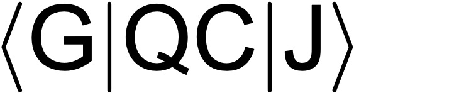
\includegraphics[height=30pt]{head_foot/journal_name}\hfill\raisebox{0pt}[0pt][0pt]{
\includegraphics[height=55pt]{head_foot/RSC_LOGO_CMYK}}\\[1ex]
      
\includegraphics[width=18.5cm]{head_foot/header_bar}}\par
    \vspace{1em}
    \sffamily
    \begin{tabular}{m{4.5cm} p{13.5cm} }

                     & \noindent\LARGE{\textbf{Constrained Unrestricted Hartree Fock and Single Excitation Configuration Interaction$^\dag$}}        \\%Article title goes here instead of the text "This is the title"
      \vspace{0.3cm} & \vspace{0.3cm}                                                                                                                \\

                     & \noindent\large{Ruben Van der Stichelen,$^{\ast}$\textit{$^{a}$} Full Name,\textit{$^{b\ddag}$} and Full Name\textit{$^{a}$}} \\%Author names go here instead of "Full name", etc.

                     &                                                                                                                               \\

                     & \noindent\normalsize{Do \emph{not} write an abstract. That will be done when the outline has matured into a completed paper.} \\%The abstrast goes here instead of the text "The abstract should be..."
    \end{tabular}

  \end{@twocolumnfalse} \vspace{1.6cm}

]
%%%END OF TITLE, AUTHORS AND ABSTRACT%%%

%%%FONT SETUP - please do not change any commands within this section
\renewcommand*\rmdefault{bch}\normalfont\upshape
\rmfamily
\section*{}
\vspace{-1cm}


% %%%FOOTNOTES%%%

\footnotetext{\textit{$^{a}$~Ghent Quantum Chemistry Group, Krijgslaan 281 (S3), B-9000 Gent, België}}
\footnotetext{\textit{$^{b}$~Corresponding author:} \texttt{firstname.lastname@ugent.be}}

% %Please use \dag to cite the ESI in the main text of the article.
% %If you article does not have ESI please remove the the \dag symbol from the title and the footnotetext below.
% \footnotetext{\dag~Electronic Supplementary Information (ESI) available: [details of any supplementary information available should be included here]. See DOI: 00.0000/00000000.}
% %additional addresses can be cited as above using the lower-case letters, c, d, e... If all authors are from the same address, no letter is required

% \footnotetext{\ddag~Additional footnotes to the title and authors can be included \textit{e.g.}\ `Present address:' or `These authors contributed equally to this work' as above using the symbols: \ddag, \textsection, and \P. Please place the appropriate symbol next to the author's name and include a \texttt{\textbackslash footnotetext} entry in the the correct place in the list.}


%%%END OF FOOTNOTES%%%

%%%MAIN TEXT%%%%


\section{Introduction}

\paragraph*{}
When thinking about chemistry, one always thinks in terms of atoms, that are bonded together in molecules. In order to correctly predict the behaviour of
thes entities we will need to know what they look like. How are the atoms aranged in a molecule? Why are they arranged in this way? The answer to these
questions lies in the Shrödinger equation, \eqref{eq:erwin}.
\begin{equation}\label{eq:erwin}
  \hat{H}\Psi = E\Psi
\end{equation}
The Shrödinger equation allows us to express the energy of a wave function. However, it is not exactly solvable for systems that contain one or more electrons,
i.e. all relevant systems. The reason for this is the repulsion that exists between two electrons. This term makes it impossible to solve the Shrödinger equation
analytically for most systems. That is why we need to make approximations. In this paper we will make use of the Hartree-Fock method, which accounts for this
interaction by means of a coulomb operator, \eqref{eq:coulomb}, which accounts for the electronic repulsion between electrons and an exchange operator,
\eqref{eq:exchange}, which accounts for stabilisation between electrons with the same spin.
\begin{equation}\label{eq:coulomb}
  \hat{J}_j\psi_i(1) = \int\psi_j(2)^*\boldsymbol{r}_{12}^{-1}\psi_j(2)d2 \psi_i(1)
\end{equation}
\begin{equation}\label{eq:exchange}
  \hat{K}_j\psi_i(1) = \int\psi_j(2)^*\boldsymbol{r}_{12}^{-1}\psi_i(2)d2 \psi_j(1)
\end{equation}
We can define an expectation value over the Hamiltonian and state that if we are in an energy minimum a small variation in the wave function will not induce a change
in energy \eqref{eq:hamexp}.
\begin{equation}\label{eq:hamexp}
  \langle\psi + \delta\psi|\hat{H}|\psi + \delta\psi \rangle = E + \delta E + \delta E^* + \delta E^2
\end{equation}
In first order we say that if $\psi$ is an eigenfunction of $\hat{H}$, $\delta E$ will equal zero. We will not go into any further detail here.
This approximation might take us a long way in the right direction, but does it take us all the way there? Here we need to introduce different methods within the
Hartree-Fock theory. Restricted Closed shell Hartree-Fock (RHF) forces the electrons into the same orbitals, thus creating doubly occupied orbitals. Even though this
picture is a chemically logical one, since in chemistry we think about electrons in pairs, physically there is no obligation for the electrons to exist in these pairs.
When we let go of the restriction, we enter the Unrestricted Hartree-Fock method (UHF). This  is no longer confined to closed shell species since it has no problem with
electrons that do not exist in pairs. However, we see that the wave function in this method does not contain the right symmetries. It paints a physical picture, yet the
chemical intuition is tossed out of the window. This phenomenon is called spin-contamination.
\paragraph*{}
In this particular paper we will take a look at the symmetry in the Hamiltonian. We know that in molecules there can be a lot of symmetry. This symmetry also exists in that
molecules Hamiltonian, and thus also in every eigenfunction. Now we can easily state that every approximation we make of these eigenfunctions must contain that same symmetry.
If we aspire to create somthing that is close to reality, but end up with something that does not have any real symmetry, we can do better. The important relation here is that
the Hamiltonian commutes with the $\hat{S}^2$ operator, meaning that these operators share a complete set of eigenfunctions. Thus an eigenfunction of the Hamiltonian must also
be an eigenfunction of $\hat{S}^2$. We can express this using a commutator \eqref{eq:commut}.
\begin{equation}\label{eq:commut}
  [\hat{H}, \hat{R}] = 0
\end{equation}
We pick the operator $\hat{R}$ as being a certain symmetry operator. Looking back at equation \eqref{eq:hamexp} and the constraint we applied, namely that $\delta E$ should
remain zero, one can wonder whether equation \eqref{eq:commut} also still holds. Is the slightly varied wave function still an eigenfunction of the symmetry operator as well?
This leads us to Löwdins symmetry dilemma \cite{Lowdin1963}. When we enforce the symmetry and the energy constraint at the same time, the minimum energy we reach is not the
global minimum. However when we drop the symmetry constraint and only enforce the energy, we will reach a lower energy, but will lose all the information with regard to the
symmetry of the system.
\paragraph*{}
We need some kind of theory to bring the best of both worlds together. One one side, we have the chemical intution in the restricted wave functions, on the other the physical
truth in the unrestricted wave functions. Roothaans Restricted Open Shell theory (ROHF)\cite{Roothaan1960} was an early attempt. As this approach is tedious and hard to implement, it 
is not very popular. However, more recently Tsuchimochi and Scuseria presented their Constrained Unrestricted Hartree Fock theory (CUHF)\cite{Scuseria2010}. A lot has been said 
already about this method\cite{Plakhutin2014, Scuseria2011}. In CUHF we se the spin-contamination to zero. In this work we will use the CUHF wave function as a reference for 
Single excitation Configuration Interaction (CIS). We will generate the single excitation energies for the CUHF wave function and compare them to the ROHF and UHF excitations of 
the same system.


In this paper we will begin by explaining the theory needed to understand the aformentioned concepts. We will then demonstrate the impact of spin-contamination using the hydrogen gas
dicossiation problem in the different Hartree-Fock modes. After that we will compare the CIS results for UHF, CUHF and ROHF. From there we will be able to verify whether it makes
sense to use CUHF as a reference next to ROHF and UHF.


\section{Theory}

\subsection{Spin-Contamination}
In general one can define the expectation value of $\hat{S}^2$ like equation \eqref{eq:spinexp}\cite{Andrews1991}.
\begin{equation}\label{eq:spinexp}
  \langle \hat{S}^2 \rangle = S_z^2 + S_z + q - \sum_{ij}^{pq} S_{ij}^2
\end{equation}
This equation holds for all systems with $q$ beta electrons and $p$ alpha electrons. When the overlap is diagonal, the last terms vanish and we are left with $S_z(S_z + 1)$.
Spin-contamination is then defined as Equation \eqref{eq:spincont}.
\begin{equation}\label{eq:spincont}
  \delta_s = \langle S^2 \rangle - S_z(S_z + 1)
\end{equation}
As a consequence, UHF suffers a lot from spin contamination. When the alpha and beta orbitals are not the same, the overlap matrix $S$ will not be diagonal. One can not expect the
last two terms in equation \eqref{eq:spinexp} to vanish, which will result in $\delta_s$ not being equal to zero. This also means that the wave function is no longer an eigenfunction
of $\hat{S^2}$, as we have seen before. We lose a quantum number and with it the symmetry of the system. We can rewrite spin-contamination as Equation \eqref{eq:spincont2}\cite{Savin2010}.
\begin{equation}\label{eq:spincont2}
  \delta_s = N_\beta - Tr(\gamma^\alpha\gamma^\beta)
\end{equation}
In this equation, $\gamma^{\alpha}$ and $\gamma^\beta$ are the one particle density matrices. In the NO basis, these matrices are block diagonal \cite{Scuseria2010}, with blocks that
can be seen in equations \eqref{eq:gammaa} and \eqref{eq:gammab}, where i corresponds to a certain closed shell orbital. The $\gamma^\alpha$ also contains a block that is a
unity matrix with dimensions $n\times n$ where n is the amount of singly occupied orbitals. In $\gamma^\beta$ this block is a zero matrix of the same dimensions.
\begin{subequations}
  \begin{align}
    \label{eq:gammaa}
    \gamma^\alpha_i & = \begin{bmatrix}
      n_i & m_i    \\
      m_i & 1- n_i
    \end{bmatrix} &  & \\
    \label{eq:gammab}
    \gamma^\beta_i  & = \begin{bmatrix}
      n_i  & -m_i  \\
      -m_i & 1-n_i
    \end{bmatrix} &  &
  \end{align}
\end{subequations}
In these equations $n_i$ is the occupation of orbital i and $m_i = \sqrt{n_i - n_i^2}$\cite{Scuseria2010}. We can the define the spin density matrix $M = (\gamma^\alpha - \gamma^\beta)/2$. It is obvious then that equation \eqref{eq:mmatrix} then holds.
\begin{equation}\label{eq:mmatrix}
  M_i = \begin{bmatrix}
    0   & m_i \\
    m_i & 0
  \end{bmatrix}
\end{equation}
Using this information we can rewrite equation \eqref{eq:spincont2} to equation \eqref{eq:spincont3}\cite{Scuseria2010}.
\begin{equation}\label{eq:spincont3}
  \delta_s = N_\beta - (N_\alpha + N_\beta)/2 + 2*Tr(M^2)
\end{equation}
In an additional step, we can use algebra to find equation \eqref{eq:spincontfinal}.
\begin{equation}\label{eq:spincontfinal}
  \delta_s = 4\sum^{N_{cp}}_i m_i^2
\end{equation}
Now if we want to make the spin contamination zero, we have to eneforce double occupation or no occupation at all. The $N_{cp}$ are the closed shell orbitals. We see here that in
the closed shell itself, we can no longer have a difference between alpha and beta orbitals. This will be the constraint that gives us the CUHF method. This method bears some 
similarities with the ROHF method in which the concept of an open shell and a closed shell part of the same wave function exist next to each other.

\subsection{Constrained Unrestricted Hartree Fock}
When talking about CUHF, there is more then one way to make sure that the spin-contamination remains zero. Scuseria and Tsuchimochi will enforce the constraint we mentioned in the
last section, where they allow only doubly occupied orbitals in the closed shell\cite{Scuseria2010}. It can be shown that the normal UHF energy can be constructed by adding a
correlation energy term to the closed shell energy. These terms can be seen in equations \eqref{eq:cseng} and \eqref{eq:correng}\cite{Savin2010}.
\begin{subequations}
  \begin{align}
    \label{eq:cseng}
    E_{cs} & = 2\sum_{ij}h_{ij}P_{ij} + \sum_{ijkl}(2\langle ij|kl\rangle - \langle ij|lk \rangle)P_{ik}P_{jl} &  & \\
    \label{eq:correng}
    E_c    & = -\sum_{ijkl}\langle ij|lk \rangle M_{ik}M_{jl}                                                  &  &
  \end{align}
\end{subequations}
Where the matrix $M$ is the spin density matrix (cfr. supra) and the $P$ matrix is the charge density matrix: $P = (\gamma^\alpha + \gamma^\beta)/2$. If we take the
derivative with respect to the density matrices we find equations \eqref{eq:der1} and \eqref{eq:der2}.
\begin{subequations}
  \begin{align}
    \label{eq:der1}
     &  & \frac{\partial E_{cs}}{\partial \gamma^\alpha_{ij}} & = \frac{\partial E_{cs}}{\partial \gamma^\beta_{ij}} = F^{cs}_{ij}                                             \\
    \label{eq:der2}
     &  & -\frac{\partial E_c}{\partial \gamma^\alpha_{ij}}   & = \frac{\partial E_c}{\partial \gamma^\beta_{ij}} = \sum_{kl} \langle ik|lj \rangle M_{kl} = \Delta^{UHF}_{ij}
  \end{align}
\end{subequations}
So in fact, the UHF Fock operators can be written as a sum of this $\Delta^{UHF}$ and the closed shell Fock operator. Now we need to expand this concept to CUHF. In general, we want
to be able to write the CUHF Fock matrix $\tilde{F}$ as the closed shell Fock matrix to which we add a certain $\Delta^{CUHF}$. As we have already seen, the constraint is only
applied to the virtual and closed shell orbitals. When we display the Fock matrix in MO basis it will exist in blocks, \eqref{eq:fockblock}. The \textit{c}, \textit{o} and \textit{v}
stand for closed shell, open shell and virtual respectively.
\begin{equation}\label{eq:fockblock}
  F = \begin{bmatrix}
    F_{cc} & F_{co} & F_{cv} \\
    F_{oc} & F_{oo} & F_{ov} \\
    F_{vc} & F_{vo} & F_{vv} \\
  \end{bmatrix}
\end{equation}
We apply the contraint in the \textit{vc} and \textit{cv} blocks. We can do this by stating that $[\tilde{F}^\sigma, \gamma^\sigma] = 0$, where $\sigma$ can equal either $\alpha$
or $\beta$. This basically means that the density matrices should share a complete set of eigenfunctions with the Fock matrices. This, in turn, means that the Fock matrices should be
diagonal at self consistent field (SCF) conditions in the NO basis. By subtracting the two conditions and algebraically working out the result we find that at SCF conditions
$\Delta^{CUHF}_{cv}$ has to be equal to zero. This means that $\tilde{F}_{cv} = F_{cv}^{cs}$\cite{Scuseria2010}. For every other block, the CUHF Fock matrix equals the UHF Fock matrix,
so the $\Delta^{CUHF}$ equals the $\Delta^{UHF}$. When we enforce this contraint during every iteration, we will decrease the spin contamination. This does entail that we will need
to transform the $\Delta^{UHF}$ to NO basis every time to enforce this constraint. This transformation will consist of two steps. First we need to transform the density matrix to
an orthonormal basis, since AO basis is often not orthonormal. (Indeed, if it were, we would not expect any bonds to form.) We choose MO basis. The MO's are defined by the
eigenvectors of the Fock operator, we will use the closed shell Fock operator. Given the Roothaan equation \eqref{eq:roothaan}.
\begin{equation}\label{eq:roothaan}
  F_{cs}C = \epsilon S C
\end{equation}
With a simple transformation, we can see that the Fock operator will become diagonal using the transformation in equation \eqref{eq:fmo}
\begin{equation}\label{eq:fmo}
  C^T F C = \epsilon C^T S C
\end{equation}
This is true, since $C^T S C$ it the unity matrix if the C matrix holds the eigenvectors of the generalised eigen value problem. To transform to NO basis, we will also need the
density matrix in the MO basis. This is not trivial, since the density matrix is ussualy defined by the coeficcient matrices C. To transform the density matrix $P$, we will need
to do a slightly different transformation. This transformation is given in equation \eqref{eq:dtrans}\cite{Declercq2020}.
\begin{equation}\label{eq:dtrans}
  P^{MO} = C^{-1}P^{AO}(C^{-1})^T
\end{equation}
We can then calculate the eigenvalues and subject the $\Delta^{UHF}$ to these transformations \eqref{eq:fulltrans}, we have easy acces to the \textit{cv} and \textit{vc} blocks.
\begin{equation}\label{eq:fulltrans}
  \Delta_{NO}^{UHF} = V^{-1} C^T \Delta^{UHF}_AO C V^{-1}
\end{equation}
The $V$ matrix containts the coefficients of the eigenvectors of the $P$ matrix. Now we just switch the required blocks to zero, backtranform and add the now $\Delta$ to the closed
shell Fock matrix.

\subsection{Configuration interaction}

The Hartree Fock approximation gives us an initial guess for the energy and the wavefunction. However, it can be improved upon. These methods are called post Hartree-Fock methods.
The difference in energy between the two methods is called the correlation energy \eqref{eq:Ecorr}.
\begin{equation}\label{eq:Ecorr}
  E_{corr} = \mathcal{E}_0 - E_0
\end{equation}
Here $E_0$ is the Hartee-Fock energy and $\mathcal{E}_0$ it the post Hartree-Fock energy. There are various approaches to post Hatree-Fock methods. We will be looking a little closer
at configuration interaction. The concept is fairly straightforward. If $\Psi_0$ is a good approximation of the wave function $\Phi_0$, we know that we can make a better approximation
using a linear combination of excited states \eqref{eq:lincomb}\cite{Szabo1996}. If all these states are called configurations, they will interact, hence the name configuration
interaction, or CI for short.
\begin{equation}\label{eq:lincomb}
  |\Phi_0\rangle = c_0|\Psi_0\rangle + \sum_{ar}|\Psi_a^r\rangle + \sum_{a<b,r<s}c_{ab}^{rs}|\Psi^{rs}_{ab} \rangle + \cdots
\end{equation}
With regard to this new wave function $\Phi_0$ we can observe some interesting phenomena. When we try to get the energy expectation value of this function, we can write it in matrix
form, where each row and collumn correspond to a certain excited state. When we look at single excitations, so at stats $\Psi_r^a$ where the electron from orbital $r$ has been
excited to orbital $a$, we can write equation \eqref{eq:overlapsingle}\cite{Szabo1996}.
\begin{equation}\label{eq:overlapsingle}
  \langle\Psi_0 |\hat{H}|\Psi_r^a\rangle = \langle a|h|r \rangle + \sum_b \langle ab||rb \rangle = \langle \chi_a |\hat{f}| \chi_r \rangle = F_{ra}
\end{equation}
Here $\langle ab||rb \rangle$ is shorthand notation for $\langle ab | rb \rangle - \langle ab | br \rangle$. The letter a here represents the orbital $\chi_a$
Now of course, by definition, at SCF conditions the off diagonal elements of the Fock matrix are zero. This is known as Brillouin's theorem. It states that there is no overlap
between single excited states and the ground state wave functions when taking the expectation value over the Hamiltonian. This makes sense, because if there was, the ground state
would not be the most stable in the first place. What this means is that when only looking at single excitations, we do not expect to see the energy lowered. And indeed, one can
prove equation \eqref{eq:doubles}\cite{Szabo1996}. The correlation energy is only defined by the overlap between second order excited states.
\begin{equation}\label{eq:doubles}
  E_{corr} = \sum_{i<j, r<s} C_{ij}^{rs}\langle \Psi_{0} |\hat{H}|\Psi_{ij}^{rs}\rangle
\end{equation}
In CIS we are only interested in the first order excitations. This might seem odd, since we do not excpect a more stable wave function. However, it can give us information about the
excited states and the excitation energies that come with them. Now we are interested in the expectation values over the Hamiltonian of all the exited states, so we need an expression
for $\langle \Psi_r^a |\hat{H}| \Psi_s^b \rangle$. There are four different situations that we need to discuss here\cite{Sherrill1996}. The first scenario is an excitation where
$a \neq b$ and $r \neq s$. The only term that will remain in that case is $\langle aj || ib \rangle$. Another case is when $r = s$ but $a \neq b$. Then the matrix element can be
expressed using equation \eqref{eq:exp1}
\begin{equation}\label{eq:exp1}
  \langle \Psi_r^a|\hat{H}|\Psi^b_r \rangle = h_{ab} + \sum_{k\in r} \langle ak || bk \rangle = F_{ab} - \langle ar||br \rangle
\end{equation}

Another case, where $r \neq s$ and $a = b$ we can write equation \eqref{eq:exp2}.
\begin{equation}\label{eq:exp2}
  \langle \Psi_r^a|\hat{H}|\Psi^a_s \rangle = -h_{rs} - \sum_{k \in \{\Psi_0 + a\}} \langle ak || bk \rangle = -F_{rs} - \langle ra || sa \rangle
\end{equation}
Finally when both $a = b$ and $r = s$ we can find \eqref{eq:exp3}
\begin{multline}\label{eq:exp3}
  \langle \Psi^a_r|\hat{H}|\Psi^a_r \rangle = \sum_{k \in \Psi_0}h_{kk} + \frac{1}{2}\sum_{k,l \in \Psi_0} \langle kl||kl \rangle - h_{rr} + h_{aa} \\ - \sum_{k \in \Psi_0} \langle
  kr || kr \rangle + \sum_{k \in \Psi_0} \langle ka||ka \rangle - \langle ra||ra \rangle
\end{multline}
We can pull all these equations into one general equation \eqref{eq:matrixelement}.
\begin{equation}\label{eq:matrixelement}
  \langle \Psi_r^a|\hat{H}|\Psi_s^b \rangle = E_0\delta_{rs}\delta_{ab} + F_{ab}\delta_{rs} - F_{rs}\delta_{ab} + \langle as || jb \rangle
\end{equation}
We notice that $E_0$ is added along the diagonal. Since we know that the trace of a matrix is equal to the sum of its eigenvalues, we can subtract $E_0$ from the diagonal and just
add it to every eigenvalue at the end. At self consistent field conditions the Fock operator equals $F_{ij} = \epsilon_i\delta_{ij}$, so Equation \eqref{eq:matrixelement} can be
simplified to equation \eqref{eq:simple}.
\begin{equation}\label{eq:simple}
  \langle \Psi_r^a|\hat{H}|\Psi_s^b \rangle = (\epsilon_a - \epsilon_r)\delta_{rs}\delta_{ab} + \langle as || jb \rangle
\end{equation}
The $\epsilon$ values correspond to the orbital energies. If we now diagonilize this matrix we end up with the excitation energies and contributions of the single excited states as
eigenfunctions. However, since electrons in alpha orbitals can be excited to beta orbitals, which is especcially important in UHF, we have to do some extra steps, using the
Kronecker product \eqref{eq:kron}.
\begin{equation}\label{eq:kron}
  R' = I_2 \otimes (I_2 \otimes R)^T
\end{equation}
The $R'$ matrix now has double the dimensions of the original R matrix. This is necesarry for the two electron integrals, since they only contain half the orbitals. These integrals
are in the original basis, but we need to account for all possible excitations, meaning that we have to account for alpha and beta orbitals at the same time. Since the two electron
integrals are given in AO basis, they still need to be transformed to MO basis, since we want the Fock operators to be diagonal in Equation \eqref{eq:matrixelement}. To do this
transformation we will need the coefficient matrix from Equation \eqref{eq:coefs}.
\begin{equation}\label{eq:coefs}
  C' = \begin{bmatrix}
    C_a & 0   \\
    0   & C_b \\
  \end{bmatrix}
\end{equation}
In this matrix $C_a$ corresponds to the coefficient matrix of the alpha orbitals and $C_b$ to the coeficient matrix of the beta orbitals. The diagonal blocks are all zero, since there
is no contibution of the alpha orbitals to the beta orbitals and vice versa.


\section{Methodology}
\label{sec:method}
The RHF, UHF and CUHF algorythms were implemented in the programming language python. We used the packages numpy, scipy and psi4. Numpy and scipy deliver tools for matrix manipulation
and other linear algebra calculations that we had to do. Psi4 is an open source quantum chemistry package allows us to calculate certain properties of the system given a molecular
geometry. These properties include nuclear repulsion, kinetic energy of the electrons among others. It also allows us to generate reference data for the molecular energy in RHF, UHF
and CUHF. It also features a method for calculating ROHF energies. They also present the possiblility to do configuration interaction for RHF and ROHF. The CIS reference data for
UHF and CUHF were generated using the GQCP library.
\paragraph*{}
For CIS $H_3$ will be used as a model system. Firstly because it it a simple system containing few electrons. This means that we do not need to track a lot of possible excitations, so
the focus can shift towards the interpretation. For this same reason we will pick the STO-3G basis set. This set provides us with the minimal amount of basis functions needed to
describe the system. This again makes interpretation the key point. We also note that $H_3$ is an open shell system, so that our results might be extrapolated to other open shell
sytems.
\section{Results and discussion}
\label{sec:results}

\subsection{$H_2$ Stretch}
\label{subsec:h2}
To demonstrate the impact of spin contamination and the importance of finding methods to overcome it, we will discuss the hydrogen gas dissociation problem\cite{Szabo1996}. Hydrogen
gas is a molecule that can be described perfectly by RHF. However, when we stretch the bond the system evolves to a state of separate hydrogen atoms. These can of course not be
described by RHF and so we expect the RHF energy to be totaly unrealistic at large bond lengths. This can be observed in figure \ref{fig:rhfstretch}.
\begin{center}
  \begin{figure}[h]
    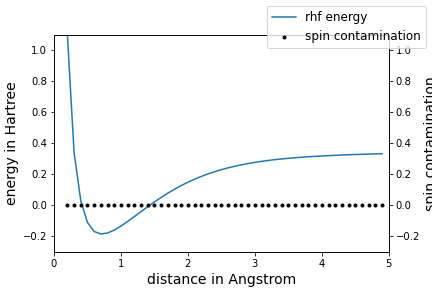
\includegraphics[width=\linewidth]{./../notes/figures/rhf.png}
    \caption{The RHF energy against the distance in an $H_2$ stretch. The zero level was chosen as the energy of two separate hydrogen atoms.}
    \label{fig:rhfstretch}
  \end{figure}
\end{center}
We can see that the RHF energy does not behave as we would expect it to. Indeed, we expect the energy to evolve towards the energy of two seperate hydrogen atoms, which clearly does
not happen. This is because the physical picture we are seeing is intrinsically invalid. The RFH algorithm forces the electrons into the same orbital, the bonding orbital between
the two nuclei. However, when the bond length increases, we expect the electrons to each be in their own respective orbitals around a single nucleus. At a distance of infinity, they
should find themselves in a normal hydrogen s orbital. RHF is too limited and does not allow this. Worth noting is that the spin contamination remains zero all the way. This means
that the wave function is an eigenfunction of the $\hat{S}^2$\cite{Scuseria2011}. \\
We want to improve this image by using UHF.  When we drop the constraint that the alpha and beta orbitals must be identical we can indeed expect the energy to behave like we expect
it to. But since $H_2$ is a closed shell system we need to do a little manipulation before starting the algorithm. When we would do a core guess, so start from the molecular
Hamiltonian as an approach for two Fock matrices, we would still find the restricted sollution. To counteract this we will need to do a mixed guess. For this we change the initial
guess for the beta electrons by mixing the Highest Occupied Molecular Orbital (HOMO) and the Lowest Unoccupied Molecular Orbital (LUMO) as a linear combination. This proces is also
known as symmetry breaking. The result can be seen in \ref{fig:uhfstretch}.
\begin{center}
  \begin{figure}[h]
    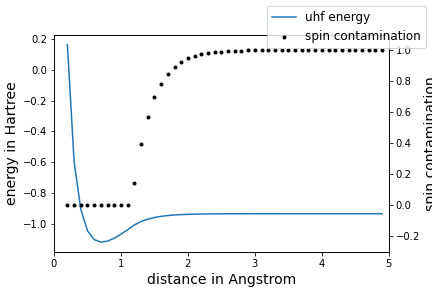
\includegraphics[width=\linewidth]{./../notes/figures/uhf.png}
    \caption{The UHF energy against the distance in an $H_2$ stretch}
    \label{fig:uhfstretch}
  \end{figure}
\end{center}
This result is physically more acurate. We see that the system does evolve towards two separate hydrogen atoms. However, the spin contamination is rising, and after a certain point
reaches the value one. This means that the wave function does no longer have the right symmetry. And as stated before, even if we cannot calculate the exact wave function we do know
what symmetries it should have. Even though we might have a lower energy energy, the wave function is not as good as an approximation as it could be\cite{Scuseria2013}. \\
This is a prime example of the aformentioned symmetry dilemma by Löwdin. If we want the lowest possible energy, we lose the symmetry. If we want to keep the symmetry, we will not
have the lowest energy. Now what would happen if we applied CUHF to the dissociation problem? This result has been plotted in \ref{fig:cuhfstretch}.
\begin{center}
  \begin{figure}[h]
    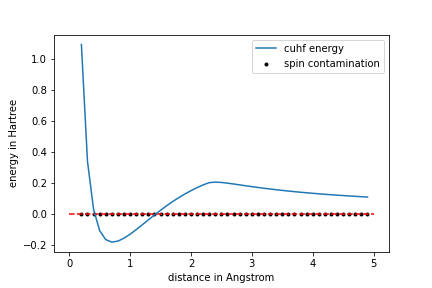
\includegraphics[width=\linewidth]{./../notes/figures/cuhf_mix.png}
    \caption{The CUHF energy against the distance in an $H_2$ stretch}
    \label{fig:cuhfstretch}
  \end{figure}
\end{center}
The CUHF picture is difficult to interpret. We see that the spin contamination remains zero. The energy seems to follow the RHF pattern (see also Figure \ref{fig:combo}) untill a
certain point, then it starts to exponentially decline. Physically this seems like a logical behaviour, as it is now again evolving to two separate hydrogen atoms. We can also notice
that the spin contamination is zero everywhere, so the symmetry of the sollution is also correct. For this plot a mixed guess was applied. In CUHF the mixed guess is done on the
active space, wich consists the orbitals to which the constraints are not applied, i.e. the open shell\cite{Scuseria2011}. So when we would take the active space as all the electrons
we reach the UHF sollution. When we take only unpaired electrons as the active space we see the ROHF sollution.
\begin{center}
  \begin{figure}[h]
    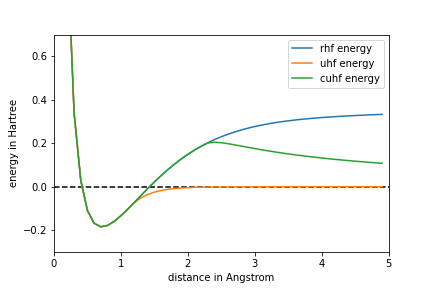
\includegraphics[width=\linewidth]{./../notes/figures/combo.png}
    \caption{The stretch energies plotted together}
    \label{fig:combo}
  \end{figure}
\end{center}
For comparison we plotted all the stretches in one plot, Figure \ref{fig:combo}. Here we can see that they all describe short bond lengths correctly, but as the internuclear distance
increases, there are deviations visible. As one would expect, the CUHF energy is able to describe short bond lengths as correctly as both RHF and UHF. While RHF deviates from the
true physical value at long bon distances, we see that CUHF does follow the expected limits (going to zero at infinity) while keeping the symmetry intact. However we see that it still
does not describe the actuall situation with a hundred percent accuracy.
\subsection{CIS results}
\label{subsec:cis}
We will compare the CIS results for $H_3$ as generated by our implementation and the one used by psi4 and GQCP. GQCP will generate the data for CUHF and UHF and Psi4 will generate
the data for ROHF. In $H_3$ we can consider nine excitations in total, so when we include the ground state, we should have ten states in total. We can take a closer look at
\ref{fig:h3_cis}.
\begin{center}
  \begin{figure}[h]
    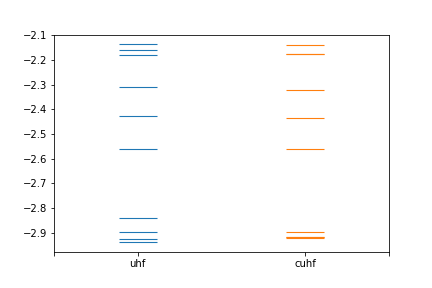
\includegraphics[width=\linewidth]{./../notes/figures/h3_cis.png}
    \caption{The CIS excitation energies for both UHF and CUHF as plotted by our implementation}
    \label{fig:h3_cis}
  \end{figure}
\end{center}
When we look at the UHF energies, we can effectively count the ten values we expect. In CUHF we only count eight energies. It seems that we have some degeneracies in the CUHF
wave function. We can take a look at the table \ref{tab:excits}.
\begin{table}[h]
  \caption{The electronic excitation energies of $H_3$ in STO-3G basis. The energy is given in Hartree.}
  \label{tab:excits}
  \begin{tabular}{l|l|l}
       & UHF       & CUHF      \\
    \hline
    1  & -2.938139 & -2.922658 \\
    2  & -2.923512 & -2.915707 \\
    3  & -2.896022 & -2.915707 \\
    4  & -2.840079 & -2.895707 \\
    5  & -2.560947 & -2.560947 \\
    6  & -2.428072 & -2.436524 \\
    7  & -2.309793 & -2.323014 \\
    8  & -2.179570 & -2.176621 \\
    9  & -2.160308 & -2.176621 \\
    10 & -2.137036 & -2.139049
  \end{tabular}
\end{table}
We do indeed notice that energies two and three are equal, as well as the energies eight and nine. Of course it is logical to find a UHF result where all the expectation values are
different. If all orbitals are different, it is logical that an electron will not encounter the same energy barrier twice. However in CUHF we discover that there are some identical
excitation energies. We know that the CUHF wave function should obey the constraint, and since all excited states are eigenfunctions of the same Fock operators, we expect them to
obey the constraint as well. However, something odd might be noticed here. The lowest excitation does not equal the ground state. When we consult our data in table 
\ref{tab:ground states}, we notice that the lowest excitation is lower in energy then the ground state.
\begin{table}[h]
  \caption{Electronic ground state energies for $H_3$ in the STO-3G basis. The energy is given in Hartree.}
  \label{tab:ground states}
  \begin{tabular}{l|l|l}
                        & UHF       & CUHF      \\
    \hline
    ground state energy & -2.923512 & -2.915707
  \end{tabular}
\end{table}
This data was verified using the GQCG library. This appears very odd, since Brillouin's theorem clearly states that the ground state expectation value over the Hamiltonian
does not mix with the first order excited states. Somehow Brillouins theorem seems not to hold in CUHF, and UHF as well for that matter. Now we need to compare it to ROHF theory. 
The Psi4 reference data for ROHF generates two states, one of which is the ground state. The energies are given in table \ref{tab:ROHF}.
\begin{table}[h]
  \caption{Electronic excitation energies of $H_3$ in ROHF according to psi4. The energy is given in Hartree.}
  \label{tab:ROHF}
  \begin{tabular}{l|l}
    & energy \\
    \hline
    1 & -2.915707 \\
    2 & -2.176621
  \end{tabular}
\end{table}
We can see that the ground state energy is the same as CUHF method. However the single excitation can also be seen returning in the CUHF excitations. It is one of the doublets.
Worth noting is that ROHF does not have a predefined set of operators. In this original work, Roothaan writes about coupling coefficients that vary between cases\cite{Roothaan1960}.
Plakhutin lists a table of possible values for these coefficients\cite{Plakhutin2014}. Depending on the coefficients uses, we expect different orbital energies, so we can also
expect different excitation energies.


\section{Conclusions}
In this report we have seen that spin contamination complicates the interpretation of the UHF wave function even though it reaches the lowest possible energies. We have looked at 
CUHF thoery as a way to deal with this spin contamination. We have used it as a reference for a CIS treatment, where we have seen that it does not obey Brillouins theorem.
We have noticed that CUHF displays multiplets in its excitation energies, which points in the direction that a symmetry of the system that is left intact. A possibility for a 
next step is full CI using the CUHF wave function. When a true correlation energy is present, we could do a stretch of $H_2$ in order to see wheter we can get the symmetry and 
the energy right at the same time.



%%%END OF MAIN TEXT%%%

%The \balance command can be used to balance the columns on the final page if desired. It should be placed anywhere within the first column of the last page.

\balance

%If notes are included in your references you can change the title from 'References' to 'Notes and references' using the following command:
%\renewcommand\refname{Notes and references}

%%%REFERENCES%%%
\bibliography{outline} %You need to replace "rsc" on this line with the name of your .bib file
\bibliographystyle{aip} %the AIP's .bst file

\end{document}
